% !TEX program = lualatex
% Compile from 2026/week5; the figures used below live in figures/.
% Source: ../../2025/week5/week5.pdf (23 slides) and week5.ipynb.
\documentclass[12pt,aspectratio=43]{beamer}
% Shared Beamer design. Load after \documentclass using \input.
% Engine: LuaLaTeX. Fonts: UD Digi Kyokasho N (regular/bold), Arial.
\usepackage{luatexja-fontspec}
\setmainjfont[BoldFont={UD Digi Kyokasho N Bold}]{UD Digi Kyokasho N}
\setsansjfont[BoldFont={UD Digi Kyokasho N Bold}]{UD Digi Kyokasho N}
\setmonojfont[BoldFont={UD Digi Kyokasho N Bold}]{UD Digi Kyokasho N}
% Liberation Sans keeps the layout usable on systems without Arial.
\IfFontExistsTF{Arial}{
  \setmainfont{Arial}
  \setsansfont{Arial}
  \setmonofont{Arial}
}{
  \setmainfont{Liberation Sans}
  \setsansfont{Liberation Sans}
  \setmonofont{Liberation Sans}
}
\renewcommand{\kanjifamilydefault}{\gtdefault}

% Typeset mathematics with a dedicated TeX math font, independent of Arial.
\usefonttheme{professionalfonts}
\usepackage[mathrm=sym]{unicode-math}
\setmathfont{Latin Modern Math}
\setoperatorfont{\symup}

\definecolor{courseblue}{HTML}{4472C4}
\definecolor{ruleblue}{HTML}{8FAADC}
\setbeamercolor{normal text}{fg=black,bg=white}
\setbeamercolor{structure}{fg=courseblue}
\setbeamercolor{frametitle}{fg=black,bg=white}
\setbeamercolor{title banner}{fg=white,bg=courseblue}
\setbeamerfont{frametitle}{size=\fontsize{18}{22}\selectfont,series=\mdseries}
\setbeamerfont{quote}{shape=\upshape}
\setbeamersize{text margin left=9mm,text margin right=9mm}
\setbeamertemplate{navigation symbols}{}
\setbeamercolor{page number}{fg=gray,bg=white}
\setbeamertemplate{footline}{%
  \begin{beamercolorbox}[wd=\paperwidth,ht=2.5mm,dp=1.5mm]{page number}
    \hfill{\fontsize{8}{9}\selectfont
      \ifnum\value{framenumber}>0
        \insertframenumber\,/\,\inserttotalframenumber
      \fi}\hspace*{3mm}
  \end{beamercolorbox}}
\setbeamertemplate{headline}{%
  \hfill\textcolor{gray}{\fontsize{6}{7}\selectfont
    \hypersetup{linkcolor=gray}% Keep Beamer's title links in the header color.
    \ifnum\value{framenumber}=0 \insertshortdate\enspace\fi
    \insertshorttitle\space\insertshortsubtitle}\hspace{2mm}\vspace{1.5mm}}
\setbeamertemplate{frametitle}{%
  \vspace{2mm}\centering\insertframetitle\par
  \vspace{-1mm}{\color{ruleblue}\rule{.44\paperwidth}{.5pt}}\par
  \vspace{2mm}}
\setbeamercolor{itemize item}{fg=courseblue}
\setbeamercolor{itemize subitem}{fg=black}
\setbeamercolor{itemize subsubitem}{fg=black}
\setbeamertemplate{itemize item}{\textbullet}
\setbeamertemplate{itemize subitem}{\textnormal{-}}
\setbeamertemplate{itemize subsubitem}{\textnormal{-}}
\setlength{\parskip}{.45em}
\hypersetup{colorlinks=true,urlcolor=courseblue}

% Use \titlepage inside a [t,noframenumbering] frame. The background extends
% 1 mm past both page edges to avoid hairline gaps in PDF viewers.
\setbeamertemplate{title page}{%
  \vspace{2mm}
  \begin{beamercolorbox}[wd=\paperwidth,ht=43mm,dp=13mm,colsep*=1mm,center]{title banner}
    {\fontsize{32}{40}\selectfont\inserttitle\par}
    \vspace{2mm}
    {\fontsize{20}{24}\selectfont\insertsubtitle\par}
  \end{beamercolorbox}
  \vspace{10mm}
  \hfill\insertauthor
}

\graphicspath{{figures/}}
\usepackage{listings}
\usepackage{upquote}
\IfFontExistsTF{Consolas}{\newfontfamily\codefont{Consolas}}{\newfontfamily\codefont{Liberation Mono}}
\definecolor{codevalue}{HTML}{7A3E9D}
\definecolor{codebuiltin}{HTML}{006DB0}
\definecolor{codestring}{HTML}{267348}
\newcommand{\code}[1]{{\codefont #1}}

\lstdefinestyle{python}{
  language=Python,
  basicstyle=\codefont\fontsize{12}{14}\selectfont,
  keywordstyle=\color{codebuiltin},
  keywordstyle=[2]\color{codebuiltin},
  morekeywords=[2]{print,range},
  stringstyle=\color{codestring},
  showstringspaces=false,
  columns=fullflexible,
  keepspaces=true,
  upquote=true,
  tabsize=4,
  breaklines=false,
  backgroundcolor=\color{black!4},
  frame=single,framerule=0pt,framesep=1.7mm,
  xleftmargin=1.7mm,xrightmargin=1.7mm,
  aboveskip=1mm,belowskip=0.5mm,
  literate=*{0}{{{\color{codevalue}0}}}1
    {1}{{{\color{codevalue}1}}}1 {2}{{{\color{codevalue}2}}}1
    {3}{{{\color{codevalue}3}}}1 {4}{{{\color{codevalue}4}}}1
    {5}{{{\color{codevalue}5}}}1 {6}{{{\color{codevalue}6}}}1
    {7}{{{\color{codevalue}7}}}1 {8}{{{\color{codevalue}8}}}1
    {9}{{{\color{codevalue}9}}}1
}
\lstset{style=python}
\setbeamercolor{lesson note}{fg=black,bg=courseblue!9}
\newenvironment{lessonbox}
  {\begin{beamercolorbox}[wd=\linewidth,sep=1.5mm]{lesson note}}
  {\end{beamercolorbox}\par}

\title{計算物理学B}
\subtitle{第五回：データの可視化}
\author{野垣 康介、藤本 悠輝}
\date{2026/11/17}
\hypersetup{pdftitle={計算物理学B 第五回：データの可視化},pdfauthor={野垣 康介、藤本 悠輝}}

\begin{document}

% 0. 表紙
\begin{frame}[t,noframenumbering]
  \titlepage
\end{frame}

% 1. 2026年度の講義予定
\begin{frame}{講義予定}
  \setlength{\parskip}{0pt}
  2026年度 第2学期（火曜3限）
  \par\vspace{2mm}
  \begingroup\centering
    \renewcommand{\arraystretch}{1.05}
    \begin{tabular}{@{}l@{\hspace{2mm}}l@{\hspace{4mm}}l@{\hspace{2mm}}l@{}}
      10/6 & 四則演算 & 12/8 & モンテカルロ1 \\
      10/27 & 制御文（for, if） & 12/15 & モンテカルロ2 \\
      11/6（金） & 関数 & 12/22 & 微分方程式1 \\
      11/10 & 配列（NumPy） & 1/12 & 微分方程式2 \\
      \textcolor{courseblue}{\textbf{11/17}} &
      \textcolor{courseblue}{\textbf{可視化（matplotlib）}} & 1/19 & 偏微分方程式1 \\
      11/24 & 数値微分 & 1/26 & 偏微分方程式2 \\
      12/1 & 数値積分 & 2/2 & 根の探索 \\
      \multicolumn{2}{c}{\small 〜中間レポート〜} &
      \multicolumn{2}{c}{\small 〜期末レポート〜}
    \end{tabular}\par
  \endgroup
  \vspace{2mm}
  {\small
    \textcolor{courseblue}{10/20は出張で休講。}\\
    11/6（金）は火曜授業の振替。\par}
  \vspace{1mm}
  {\fontsize{7}{8}\selectfont
    日付：\href{https://www.niigata-u.ac.jp/wp-content/uploads/2025/08/schedule_2026.pdf}{令和8年度（2026）新潟大学授業暦}\par}
\end{frame}

% 2. 授業で使うリンク
\begin{frame}{授業で使うリンク}
  \begin{itemize}
    \setlength{\itemsep}{3mm}
    \item Google Colab：{\small\url{https://colab.research.google.com/?hl=ja}}
    \item 講義資料（GitHub）：{\small\url{https://github.com/nogaki/Computational_Physics_B}}
    \item 今週のノートブック：\code{2026/week5/week5.ipynb}
    \item 今週のデータ：\code{2026/week5/pulsar.csv}
  \end{itemize}
\end{frame}

% 3. GitHubからColabへ
\begin{frame}[t]{GitHubからColabへ}
  \setlength{\parskip}{0pt}
  \begin{enumerate}
    \setlength{\itemsep}{4mm}
    \item GitHubで\code{week5.ipynb}を開き、ブラウザーのURLをコピーします。
    \item Colabで「ファイル」→「ノートブックを開く」→「GitHub」を選びます。
    \item URLを貼り付けて検索し、今週のノートブックを開きます。
  \end{enumerate}
  \vspace{3mm}
  \begin{lessonbox}
    \textbf{開いたら「ドライブにコピーを保存」}\par
    \small 「ファイル」メニューから自分用のコピーを保存します。開いただけではドライブに保存されません。
  \end{lessonbox}
\end{frame}

% 4. CSVデータをアップロード
\begin{frame}[t,fragile]{CSVデータをアップロード}
  \setlength{\parskip}{0pt}
  \begin{enumerate}
    \setlength{\itemsep}{3mm}
    \item GitHubで\code{2026/week5/pulsar.csv}を開き、ダウンロードします。
    \item Colab左側の「ファイル」から\code{pulsar.csv}をアップロードします。
  \end{enumerate}
  \vspace{2mm}
  \small CSVは表のデータです。\code{pandas}を使って読み込みます。
\begin{lstlisting}
import pandas as pd
df = pd.read_csv("pulsar.csv")
\end{lstlisting}
  \small ローカルでは、ノートブックとCSVを同じフォルダに置きます。
\end{frame}

% 5. 前回への補足
\begin{frame}[t,fragile]{前回への補足：配列の各要素を処理する}
  \setlength{\parskip}{0pt}
  PythonのリストやNumPy配列に\code{for}文を使うと、要素を順に取り出せます。
\begin{lstlisting}
import numpy as np
a = np.linspace(0, 1, 50)
for value in a:
    print(value)
\end{lstlisting}
  \vspace{1mm}
  \small \code{value}には、繰り返しごとに配列\code{a}の次の要素が入ります。繰り返す処理はスペース4個で字下げします。
\end{frame}

% 6. 今日の内容
\begin{frame}[t]{今回の内容：データの可視化}
  \begin{itemize}
    \setlength{\itemsep}{3mm}
    \item matplotlibでグラフを描く
    \item 折れ線グラフで連続的な変化を見る
    \item 散布図でデータの分布や相関を見る
    \item 等高線・密度・3次元プロットで二変数関数を見る
  \end{itemize}
  \vfill
  {\footnotesize
    参考：野本拓也・是常隆・有田亮太郎『実践計算物理学』（共立出版）\\
    \url{https://github.com/vlvovch/PHYS6350-ComputationalPhysics}}
\end{frame}

% 7. matplotlib
\begin{frame}[t,fragile]{matplotlib}
  \setlength{\parskip}{0pt}
  Pythonの計算結果をグラフにするライブラリです。\code{pyplot}を\code{plt}という名前で読み込みます。
\begin{lstlisting}
import matplotlib.pyplot as plt
\end{lstlisting}
  \begin{itemize}
    \item \code{plt.figure()}：新しい図を作る
    \item \code{plt.plot(x, y)}：配列を使って描く
    \item \code{plt.show()}：図を表示する
  \end{itemize}
  \vspace{2mm}
  \small 以下のコードは主要な命令の抜粋です。軸の設定などを含む実行用コードはノートブックにあります。
\end{frame}

% 8. 数値をグラフにする
\begin{frame}[t,fragile]{数値データをグラフで見る}
  \setlength{\parskip}{0pt}
  \small \(y=\cos x\)を、\(x=0,1,\ldots,10\) radの11点で計算します。
\begin{lstlisting}
x = np.linspace(0, 10, 11)
y = np.cos(x)
plt.plot(x, y, "o")
\end{lstlisting}
  \begin{columns}[c,onlytextwidth]
    \begin{column}{.29\textwidth}
      \small
      \begin{tabular}{rr}
        \(x\) & \(\cos x\) \\
        0 & 1.000 \\
        1 & 0.540 \\
        2 & -0.416 \\
        3 & -0.990 \\
        \(\vdots\) & \(\vdots\)
      \end{tabular}
    \end{column}
    \begin{column}{.68\textwidth}
      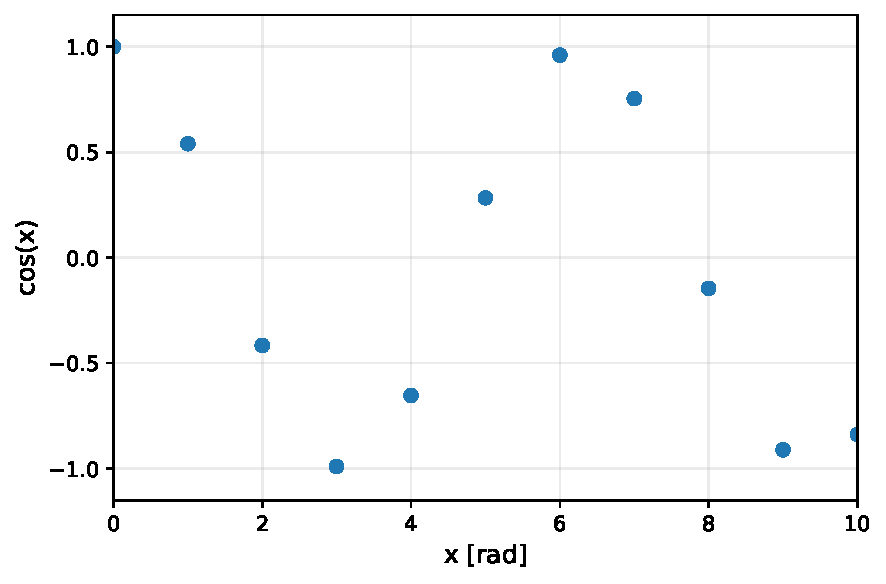
\includegraphics[width=\linewidth,height=40mm,keepaspectratio]{cos_points_11.pdf}\par
    \end{column}
  \end{columns}
\end{frame}

% 9. サンプル数を増やす
\begin{frame}[t,fragile]{計算する点を増やす}
  \setlength{\parskip}{0pt}
  \small 端点を含む101点に増やし、曲線の形を細かく表します。
\begin{lstlisting}
x = np.linspace(0, 10, 101)
y = np.cos(x)
plt.plot(x, y, "o")
\end{lstlisting}
  \centering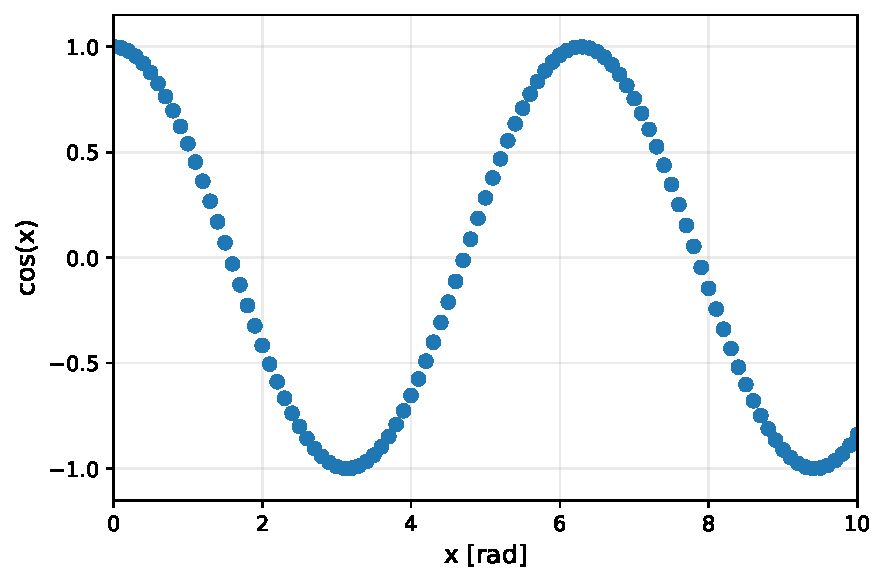
\includegraphics[height=42mm]{cos_points_101.pdf}\par
\end{frame}

% 10. 折れ線グラフ
\begin{frame}[t,fragile]{折れ線グラフ}
  \setlength{\parskip}{0pt}
  \small 隣り合う点を線分で結びます。時間や位置に沿った変化に向いています。
\begin{lstlisting}
plt.plot(x, y)
\end{lstlisting}
  \centering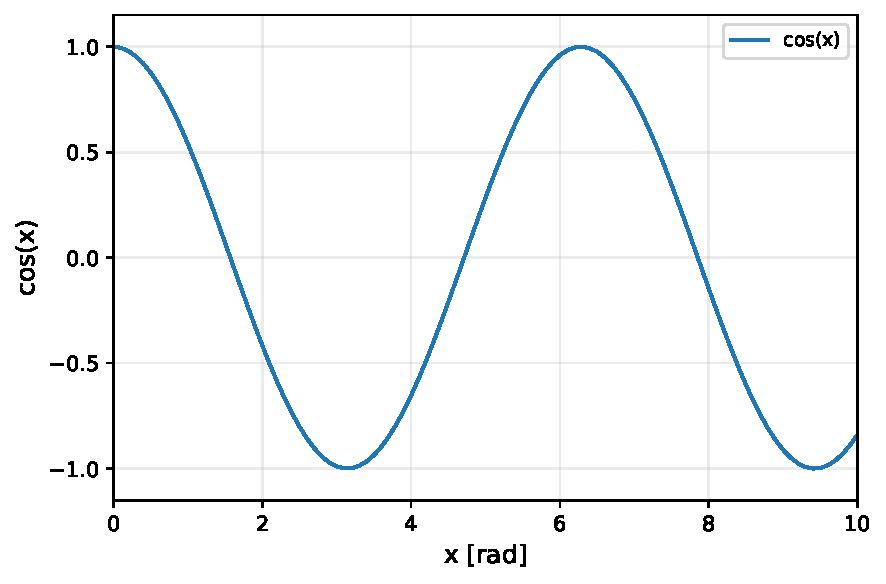
\includegraphics[height=47mm]{cos_line.pdf}\par
\end{frame}

% 11. 複数のデータ
\begin{frame}[t,fragile]{複数のデータを描く}
  \setlength{\parskip}{0pt}
  \small 凡例（\code{label}）と線種を使って曲線を区別します。
\begin{lstlisting}
plt.plot(x, y, "-", label="cos(x)")
plt.plot(x, np.sin(x), "--",
         label="sin(x)")
plt.legend()
\end{lstlisting}
  \begin{columns}[c,onlytextwidth]
    \begin{column}{.28\textwidth}
      \small 実線 \code{"-"}\\[1mm]
      破線 \code{"--"}\\[1mm]
      点線 \code{":"}\\[1mm]
      一点鎖線 \code{"-."}
    \end{column}
    \begin{column}{.70\textwidth}
      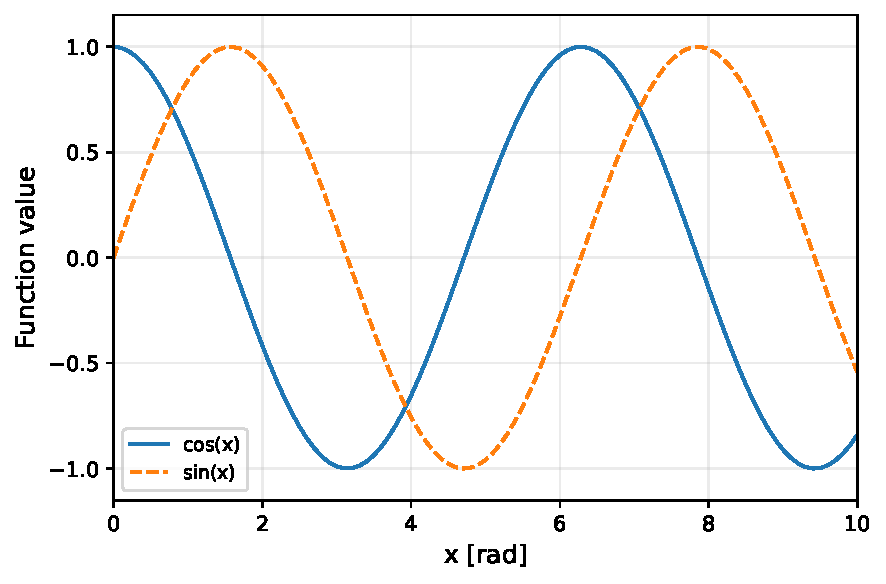
\includegraphics[width=\linewidth,height=37mm,keepaspectratio]{multiple_lines.pdf}\par
    \end{column}
  \end{columns}
\end{frame}

% 12. グラフの保存
\begin{frame}[t,fragile]{グラフをファイルに保存する}
  \setlength{\parskip}{0pt}
  \code{savefig}を使うと、レポートに使う図を保存できます。
\begin{lstlisting}
plt.figure()
plt.plot(x, y)
plt.xlabel("x [rad]")
plt.ylabel("cos(x)")
plt.savefig("graph.pdf")
plt.show()
\end{lstlisting}
  \small ファイル名の\code{.pdf}が保存形式を指定します。\code{savefig}は\code{show}より前に呼びます。Colabでは左側の「ファイル」からダウンロードできます。
\end{frame}

% 13. 点が少なすぎる例
\begin{frame}[t]{避けるべきこと：点の数が少ない}
  \setlength{\parskip}{0pt}
  \small 7点だけでは、\(\cos x\)のなめらかな変化を表しきれません。
  \par\vspace{1mm}
  \centering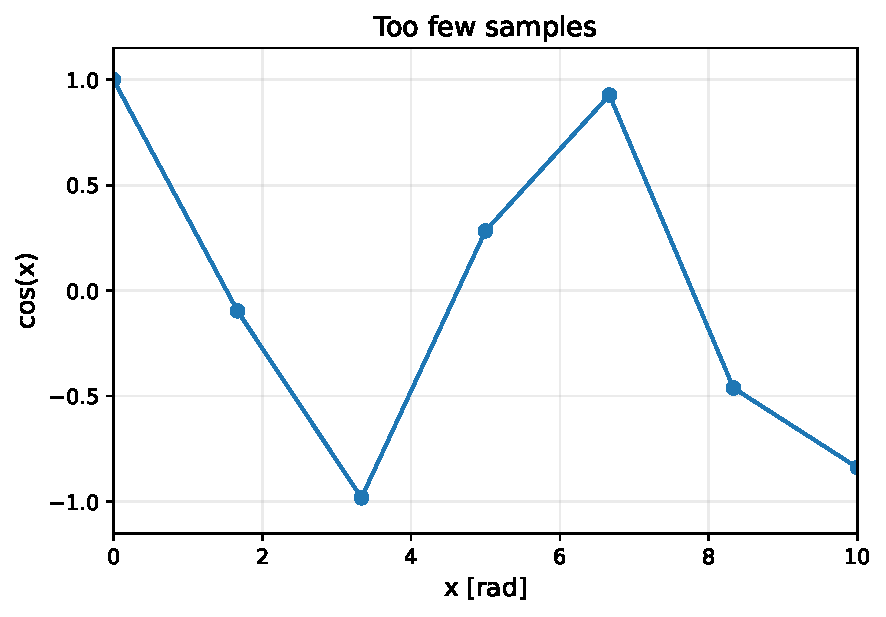
\includegraphics[height=45mm]{bad_sampling.pdf}\par
  \raggedright\small 点を増やして、図の形が十分に変わらなくなるか確認します。
\end{frame}

% 14. 軸ラベル
\begin{frame}[t,fragile]{避けるべきこと：軸ラベルがない}
  \setlength{\parskip}{0pt}
  \small 量の名前と単位を明記し、読み取れる文字の大きさにします。
\begin{lstlisting}
plt.xlabel("x [rad]")
plt.ylabel("cos(x)")
\end{lstlisting}
  \centering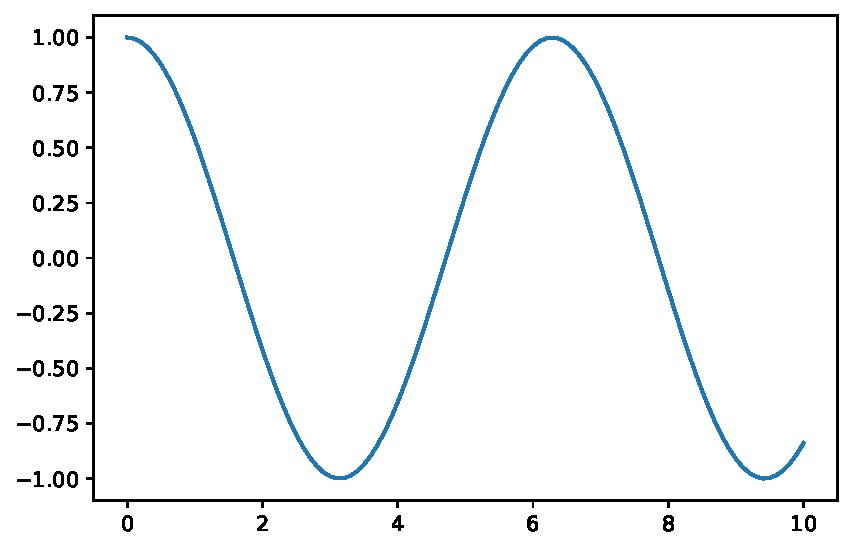
\includegraphics[height=43mm]{bad_labels.pdf}\par
\end{frame}

% 15. 線種
\begin{frame}[t]{避けるべきこと：同じ線種で重ねる}
  \setlength{\parskip}{0pt}
  \small 同じ色・線種では、凡例があっても曲線を識別しにくくなります。
  \par\vspace{1mm}
  \centering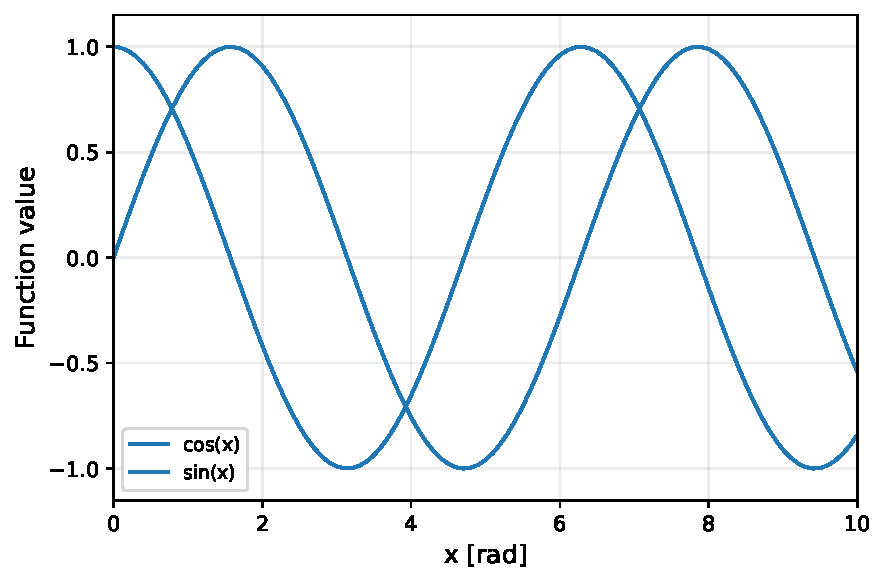
\includegraphics[height=45mm]{bad_styles.pdf}\par
  \raggedright\small 色だけに頼らず、線種やマーカーも使って区別します。
\end{frame}

% 16. 散布図
\begin{frame}[t,fragile]{散布図}
  \setlength{\parskip}{0pt}
  \small 各組\((x_i,y_i)\)を点で示し、点の分布や相関を調べます。\\
  ここではノートブックで作る模擬データを使います。
\begin{lstlisting}
plt.scatter(x_simulated, y_simulated)
\end{lstlisting}
  \centering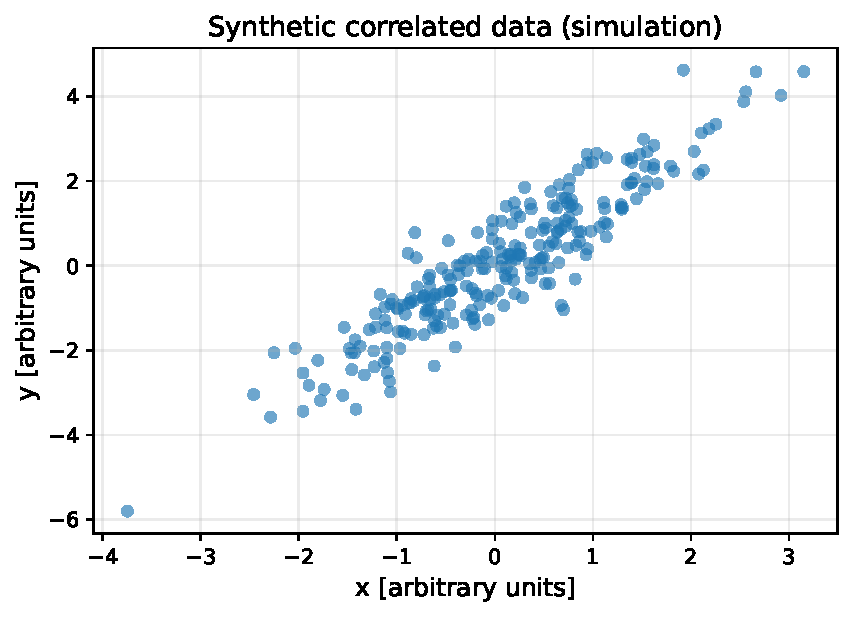
\includegraphics[height=44mm]{scatter_example.pdf}\par
\end{frame}

% 17. 粒子識別
\begin{frame}[t]{散布図の例：粒子の識別}
  \setlength{\parskip}{0pt}
  \small 運動量と物質中でのエネルギー損失を組み合わせ、粒子の種類を識別します。
  \par\vspace{1mm}
  \centering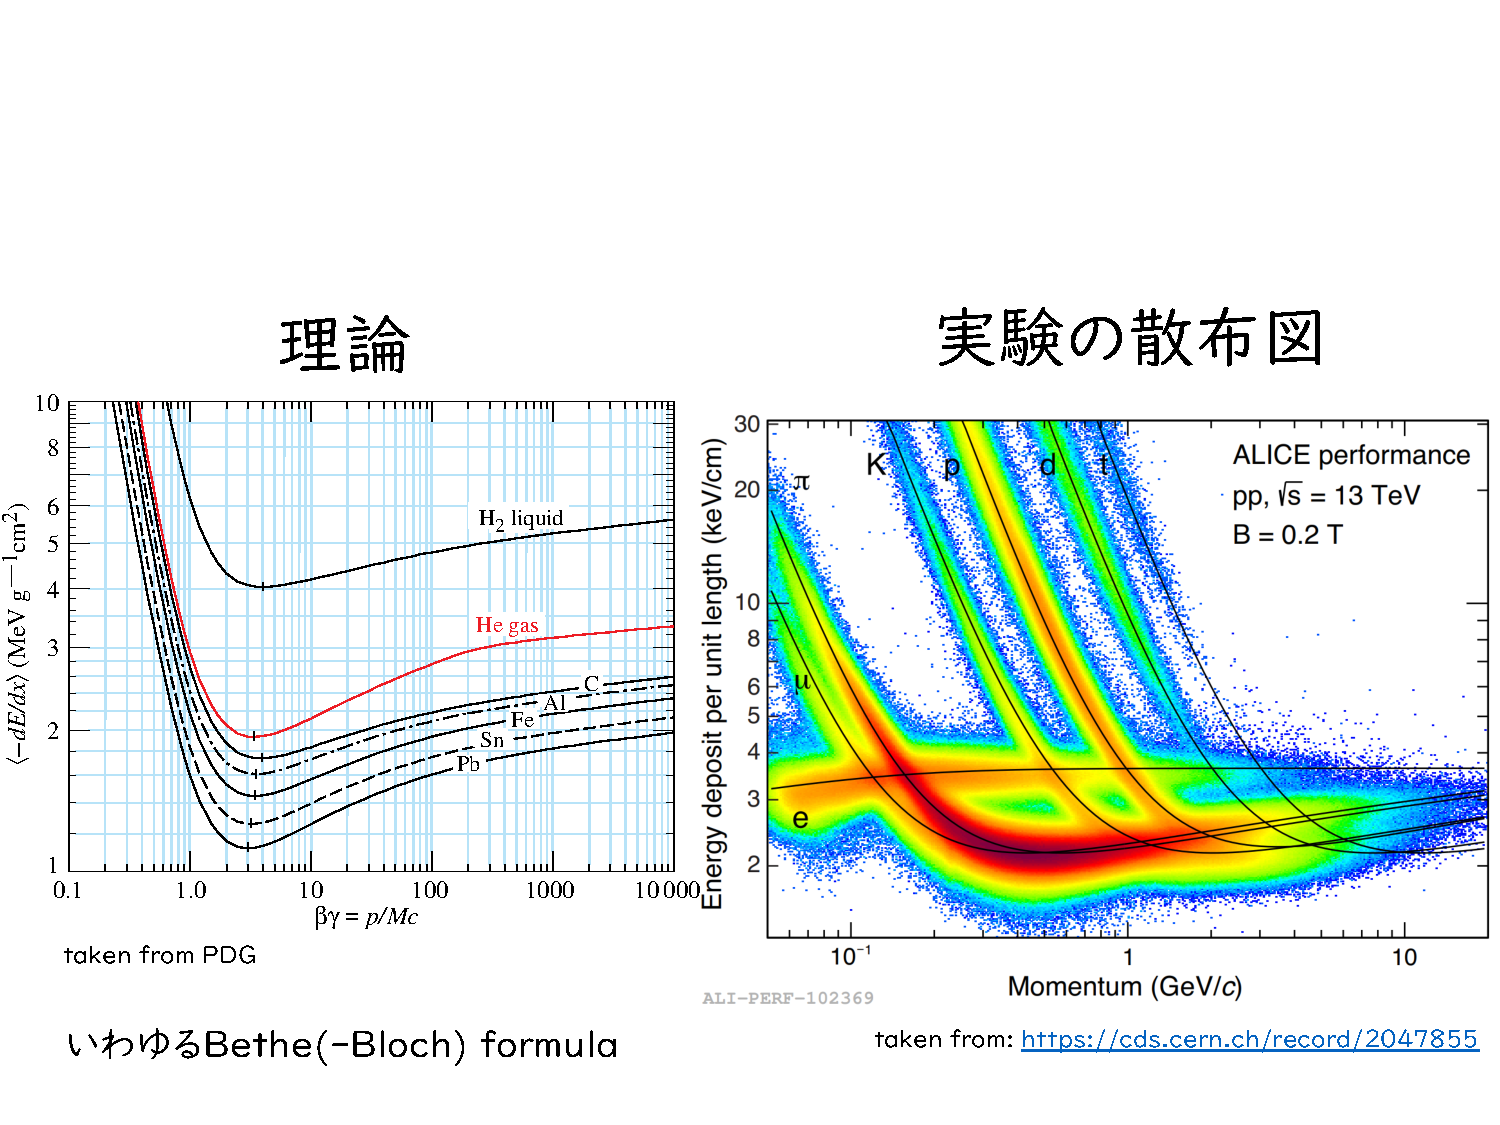
\includegraphics[width=.96\linewidth,height=46mm,keepaspectratio]{particle_identification.pdf}\par
  \raggedright{\fontsize{7}{8}\selectfont
  理論：PDG, “Passage of Particles Through Matter”。\\
  実験：ALICE Collaboration（\href{https://cds.cern.ch/record/2047855}{CERN, 2015}）。出典は元図にも表示。}
\end{frame}

% 18. パルサーの周期データ
\begin{frame}[t,fragile]{パルサーの周期と周期変化を描く}
  \setlength{\parskip}{0pt}
  \small \code{P0}は周期\(P\)（s）、\code{P1}は周期変化率\(\dot P\)（s/s）です。\code{df}は読み込んだCSVの表です。
\begin{lstlisting}
P, Pdot = df["P0"], df["P1"]
valid = np.isfinite(P)
valid &= np.isfinite(Pdot)
valid &= (P > 0) & (Pdot > 0)
plt.scatter(P[valid], Pdot[valid])
plt.xscale("log")
plt.yscale("log")
\end{lstlisting}
  \small \code{valid}がTrueの行だけを選びます。非正値も観測されますが、対数軸では表示できないため除きます。
\end{frame}

% 19. パルサーのP-Pdot図
\begin{frame}[t]{散布図の例：パルサーの周期と周期変化}
  \setlength{\parskip}{0pt}
  \centering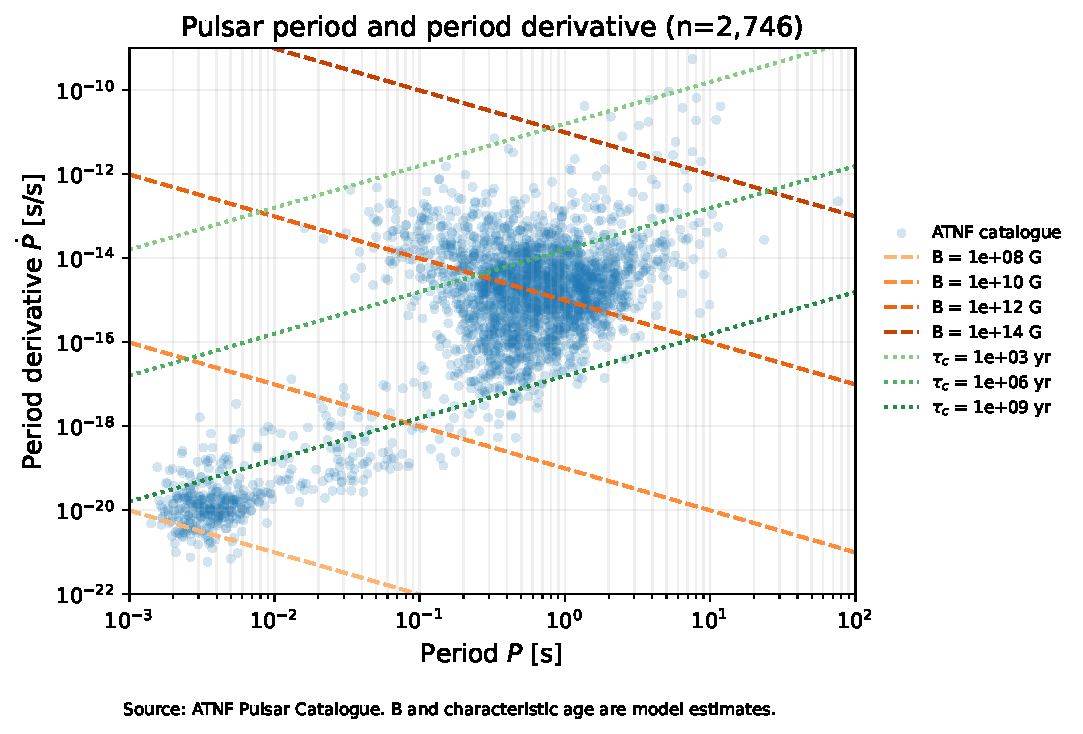
\includegraphics[height=46mm]{pulsar.pdf}\par
  \raggedright{\fontsize{9}{11}\selectfont
  破線：\(B\simeq3.2\times10^{19}\sqrt{P\dot P}\,\mathrm{G}\)、点線：\(\tau_c=P/(2\dot P)\)。\\
  \(P\)を秒で用い、\(\tau_c\)は秒から年に換算。正の内因性\(\dot P\)と磁気双極子模型を仮定した目安で、実測磁場や真の年齢ではありません。}
\end{frame}

% 20. 二変数関数の格子
\begin{frame}[t,fragile]{二変数関数を格子上で計算する}
  \setlength{\parskip}{0pt}
  \small 電気双極子の無次元ポテンシャルを例にします。正電荷を\((-2,0)\)、負電荷を\((2,0)\)に置きます。
  \[V_{\rm dip}(x,y)=\frac{1}{\sqrt{(x+2)^2+y^2}}-\frac{1}{\sqrt{(x-2)^2+y^2}}.\]
\begin{lstlisting}
x = np.linspace(-5, 5, 200)
y = np.linspace(-5, 5, 200)
X, Y = np.meshgrid(x, y)
\end{lstlisting}
  \begin{lessonbox}
    \small \code{x}, \code{y}は座標の候補です。\code{meshgrid}は各\((x,y)\)の組を格子\code{X}, \code{Y}に並べ、関数を面全体で計算できるようにします。
  \end{lessonbox}
\end{frame}

% 21. 双極子ポテンシャルを計算する
\begin{frame}[t,fragile]{双極子ポテンシャルを計算する}
  \setlength{\parskip}{0pt}
  \small 電荷の位置で発散するため、各電荷から距離0.25未満を除外します。
\begin{lstlisting}
r_plus = np.hypot(X + 2, Y)
r_minus = np.hypot(X - 2, Y)
r_plus = np.ma.masked_less(r_plus, 0.25)
r_minus = np.ma.masked_less(r_minus, 0.25)
V = 1 / r_plus - 1 / r_minus
\end{lstlisting}
  \small \code{hypot(a, b)}は\(\sqrt{a^2+b^2}\)。\code{masked\_less}は指定値未満の点を計算・表示から除外します。\code{V}の形は\code{X}, \code{Y}と同じ\code{(200, 200)}です。
\end{frame}

% 22. 等高線と塗りつぶし等高線
\begin{frame}[t,fragile]{等高線図と塗りつぶし等高線図}
  \setlength{\parskip}{0pt}
  \small \code{contour}は等しい値を線で結び、\code{contourf}は間を塗ります。
\begin{lstlisting}
levels = np.linspace(-1.5, 1.5, 13)
plt.contour(X, Y, V, levels=levels)
\end{lstlisting}
  \centering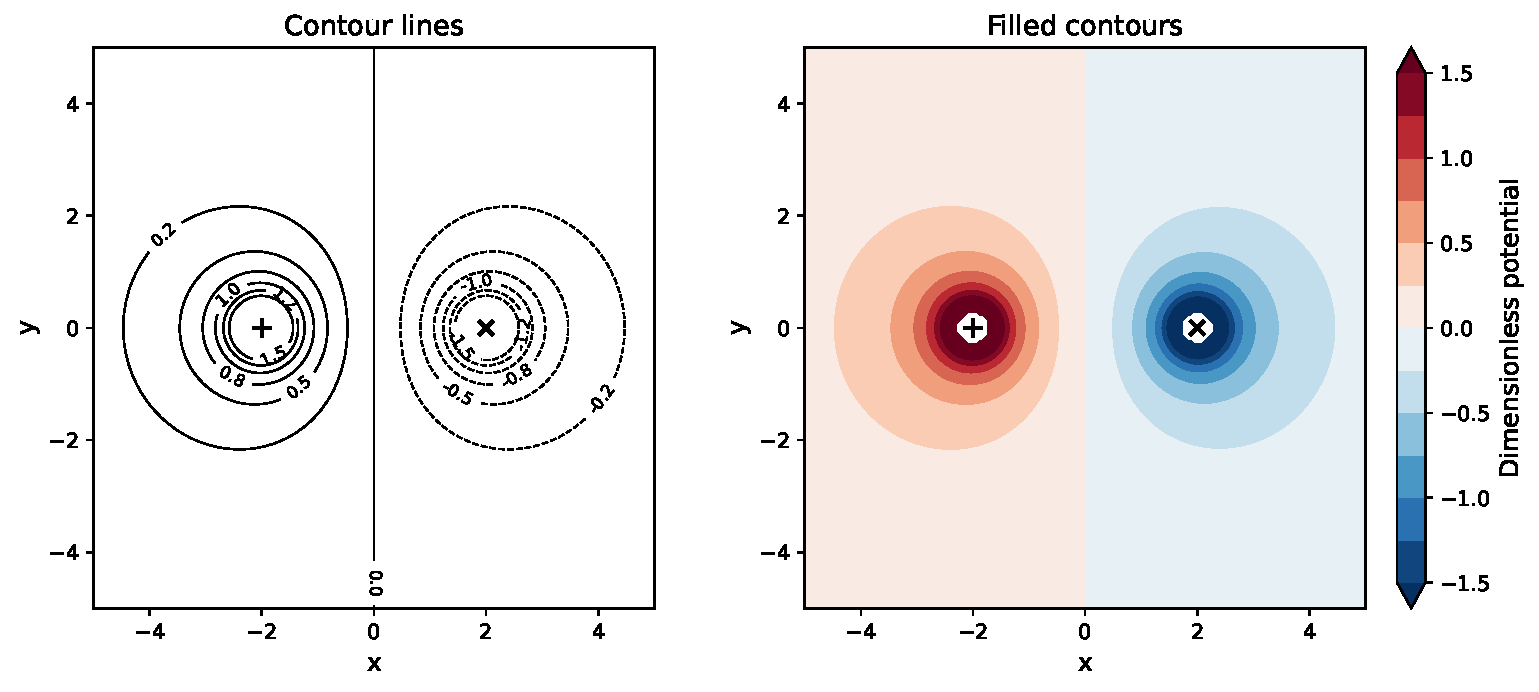
\includegraphics[width=.94\linewidth,height=38mm,keepaspectratio]{dipole_contours.pdf}\par
  \raggedright\small 左は\code{contour}、右は\code{contourf}の結果です。
\end{frame}

% 23. 密度プロット
\begin{frame}[t,fragile]{密度プロット：imshow}
  \setlength{\parskip}{0pt}
\begin{lstlisting}
plt.imshow(V, origin="lower",
           extent=[-5, 5, -5, 5],
           vmin=-1.5, vmax=1.5,
           cmap="RdBu_r")
plt.colorbar()
\end{lstlisting}
  \begin{columns}[c,onlytextwidth]
    \begin{column}{.40\textwidth}
      \small \code{extent}：座標の範囲。\\[1mm]
      \code{origin="lower"}：\(y\)の小さい側を下に。\\[1mm]
      \(\pm1.5\)を超える値は色の両端で飽和します。
    \end{column}
    \begin{column}{.58\textwidth}
      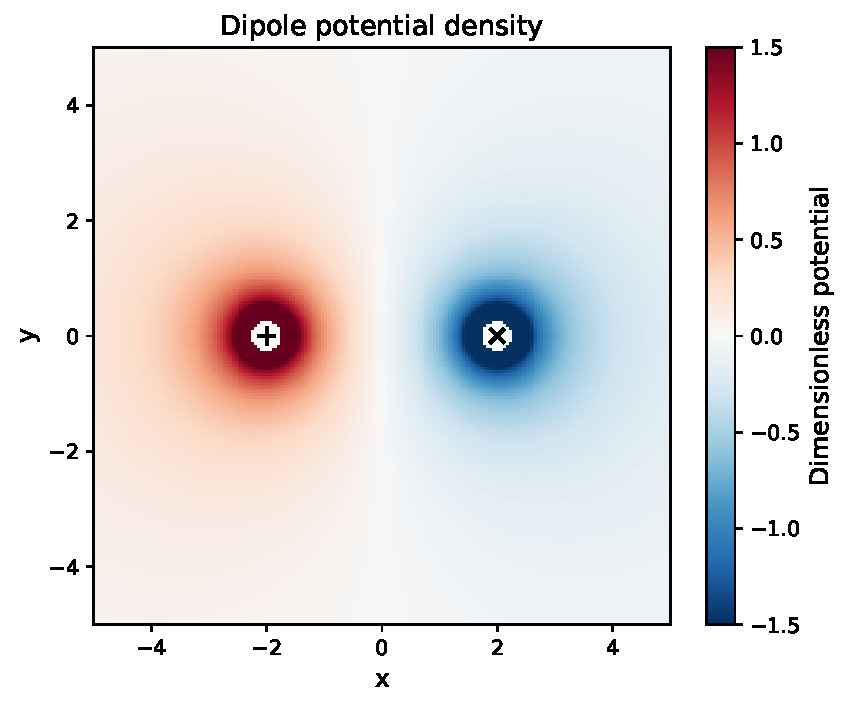
\includegraphics[width=\linewidth,height=37mm,keepaspectratio]{dipole_density.pdf}\par
    \end{column}
  \end{columns}
\end{frame}

% 24. 3次元プロット
\begin{frame}[t,fragile]{3次元プロットの作り方}
  \setlength{\parskip}{0pt}
  \small 3次元の座標軸を作り、高さを\(V(x,y)\)として曲面を描きます。
\begin{lstlisting}
fig = plt.figure()
ax = fig.add_subplot(projection="3d")
ax.plot_surface(X, Y, V,
                cmap="RdBu_r",
                vmin=-5, vmax=5)
ax.set_zlim(-5, 5)
plt.show()
\end{lstlisting}
  \small \code{fig}は図全体、\code{ax}は座標軸です。底面の等高線と視点の設定を含むコードはノートブックにあります。
\end{frame}

\begin{frame}[t]{3次元プロット：双極子ポテンシャル}
  \setlength{\parskip}{0pt}
  \centering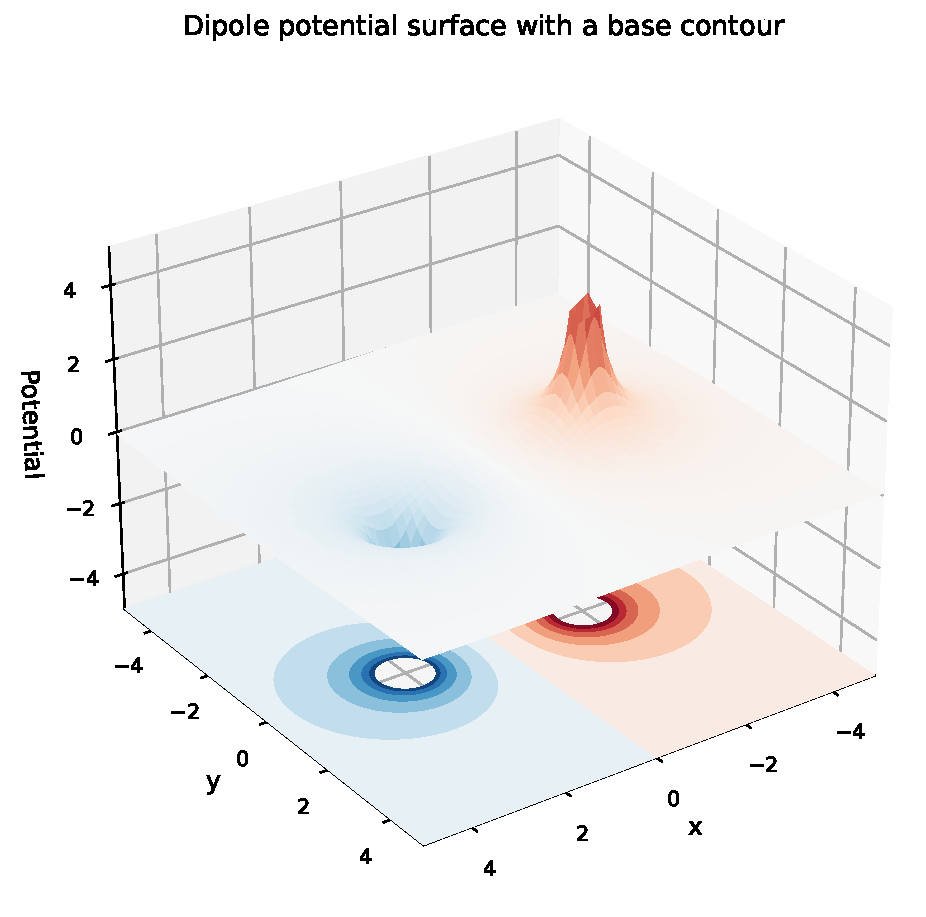
\includegraphics[height=51mm]{dipole_surface.pdf}\par
  \raggedright\small 表示範囲は\(z=-5\)〜5。白い穴は電荷の近傍を除いた部分で、電荷の位置ではポテンシャルが発散します。
\end{frame}

% 25. Bessel関数の実習
\begin{frame}[t,fragile]{実習：第一種Bessel関数を描く}
  \setlength{\parskip}{0pt}
  \small \(J_v(x)\)を\(v=0,1,2,3\)、\(0\le x\le20\)で描き、PDFに保存します。
\begin{lstlisting}
from scipy.special import jv
\end{lstlisting}
  \begin{columns}[T,onlytextwidth]
    \begin{column}{.49\textwidth}
      \small \code{v}は次数です。線種は\(v=0,1,2,3\)の順に\code{"-"}、\code{"--"}、\code{":"}、\code{"-."}とします。\\[2mm]for文で4本の曲線を描き、凡例・軸名を付けてPDFで提出します。
    \end{column}
    \begin{column}{.49\textwidth}
      \centering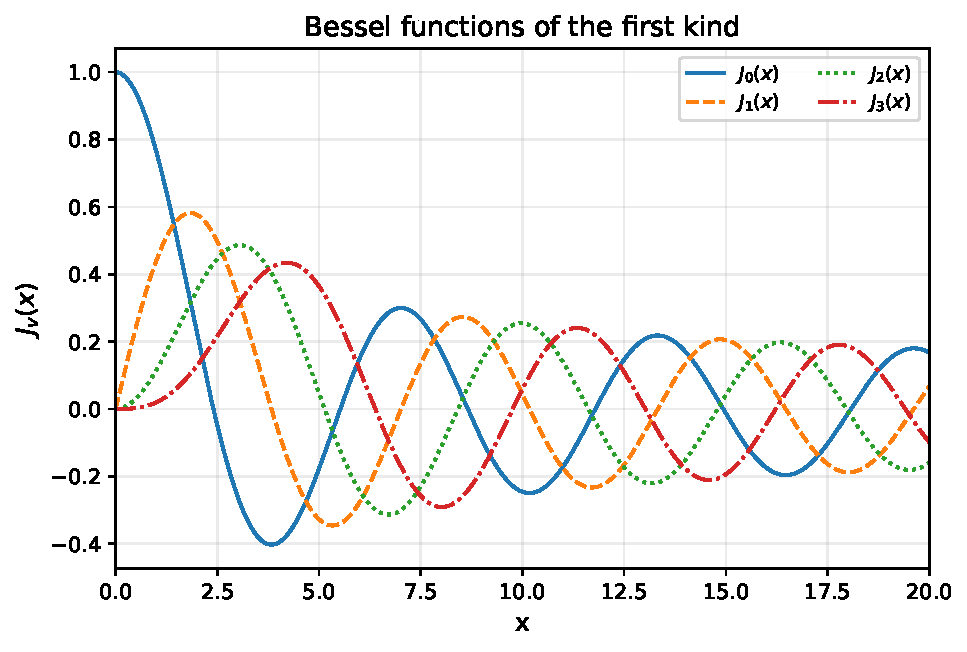
\includegraphics[width=\linewidth]{bessel.pdf}\par
    \end{column}
  \end{columns}
\end{frame}

% 26. 発展課題
\begin{frame}[t]{発展課題：フラクタルを描く}
  \setlength{\parskip}{0pt}
  次の図形から一つ選び、仕組みを調べて描いてみましょう。
  \begin{columns}[T,onlytextwidth]
    \begin{column}{.54\textwidth}
      \begin{itemize}
        \setlength{\itemsep}{1mm}
        \item マンデルブロ集合
        \item コッホ曲線
        \item バーンズリーのシダ
        \item シェルピンスキーのギャスケット
        \item ジュリア集合
      \end{itemize}
      \small さらに時間があれば、図形の変化をアニメーションにしてみましょう。
    \end{column}
    \begin{column}{.44\textwidth}
      \centering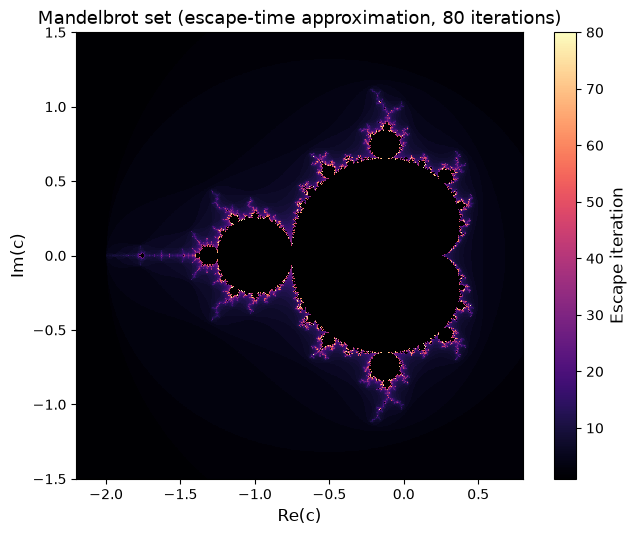
\includegraphics[width=\linewidth]{mandelbrot.png}\par
    \end{column}
  \end{columns}
\end{frame}

\end{document}
